\appendix


\section{Anhang}\label{sec:anhang}

\subsection{Code}\label{appendix:code}
Da \acs{MPS}--Code als \ac{XML} gespeichert wird, ist es nicht sinnvoll, diesen diesem Dokument beizufügen.
Deshalb wird der Code über GitHub bereitgestellt.
Das Repository ist unter folgender Adresse abrufbar: \href{https://github.com/NikBenson/BAT}{https://github.com/NikBenson/BAT}.
Der zu betrachtende Branch ist Main und die veröffentlichte Version wird den Tag {\ttfamily v1.0.0} haben.
Der Code liegt im Ordner {\ttfamily projects/} und ist ab folgendem Hash final: \enquote{98c5cb4f9d-7673803bb8-96d8e466ec-c389dd9f1b}.

\subsection{Zeitbuchungen}\label{appendix:zeitbuchungen}
\begin{table}[H]
    \centering
    \begin{tabular}{|l|c|c|}
        \hline
        Aufgabe                                & Datum      & Zeit [Stunden] \\
        \hline
        \hline
        Lernen \& \ac{JSON}--Beispiel \ac{MPS} & 19.02.2024 & 8              \\
        \hline
        Lernen \& \ac{JSON}--Beispiel \ac{MPS} & 20.02.2024 & 8              \\
        \hline
        Lernen \& \ac{JSON}--Beispiel \ac{MPS} & 21.02.2024 & 8              \\
        \hline
        Lernen \& \ac{JSON}--Beispiel \ac{MPS} & 22.02.2024 & 8              \\
        \hline
        Lernen \& \ac{JSON}--Beispiel \ac{MPS} & 23.02.2024 & 8              \\
        \hline
        Arbeit am komplexen Beispiel           & 26.02.2024 & 8              \\
        \hline
        Arbeit am komplexen Beispiel           & 27.02.2024 & 8              \\
        \hline
        Arbeit am komplexen Beispiel           & 28.02.2024 & 8              \\
        \hline
        Arbeit am komplexen Beispiel           & 29.02.2024 & 8              \\
        \hline
        Arbeit am komplexen Beispiel           & 30.02.2024 & 8              \\
        \hline
        Arbeit am komplexen Beispiel           & 29.03.2024 & 8              \\
        \hline
        Arbeit am komplexen Beispiel           & 30.03.2024 & 4              \\
        \hline
        Arbeit am komplexen Beispiel           & 01.04.2024 & 8              \\
        \hline
        Arbeit am komplexen Beispiel           & 02.04.2024 & 8              \\
        \hline
        Arbeit am komplexen Beispiel           & 03.04.2024 & 8              \\
        \hline
        Arbeit am komplexen Beispiel           & 04.04.2024 & 8              \\
        \hline
        Arbeit am komplexen Beispiel           & 05.04.2024 & 8              \\
        \hline
        Arbeit am komplexen Beispiel           & 06.04.2024 & 8              \\
        \hline
        \ac{JSON}--Beispiel \ac{POSIX}         & 11.04.2024 & 8              \\
        \hline
        \ac{JSON}--Beispiel \ac{POSIX}         & 12.04.2024 & 8              \\
        \hline
        Arbeit am komplexen Beispiel           & 15.04.2024 & 2              \\
        \hline
        Arbeit am komplexen Beispiel           & 16.04.2024 & 2              \\
        \hline
        Arbeit am komplexen Beispiel           & 15.04.2024 & 2              \\
        \hline
        Arbeit am komplexen Beispiel           & 20.04.2024 & 4              \\
        \hline
        Arbeit am komplexen Beispiel           & 22.04.2024 & 2              \\
        \hline
    \end{tabular}
    \caption{Zeitbuchungen}
    \label{tab:zeitbuchungen-long}
\end{table}

\subsection{Befragungsergebnisse}\label{appendix:befragungsergebnisse}
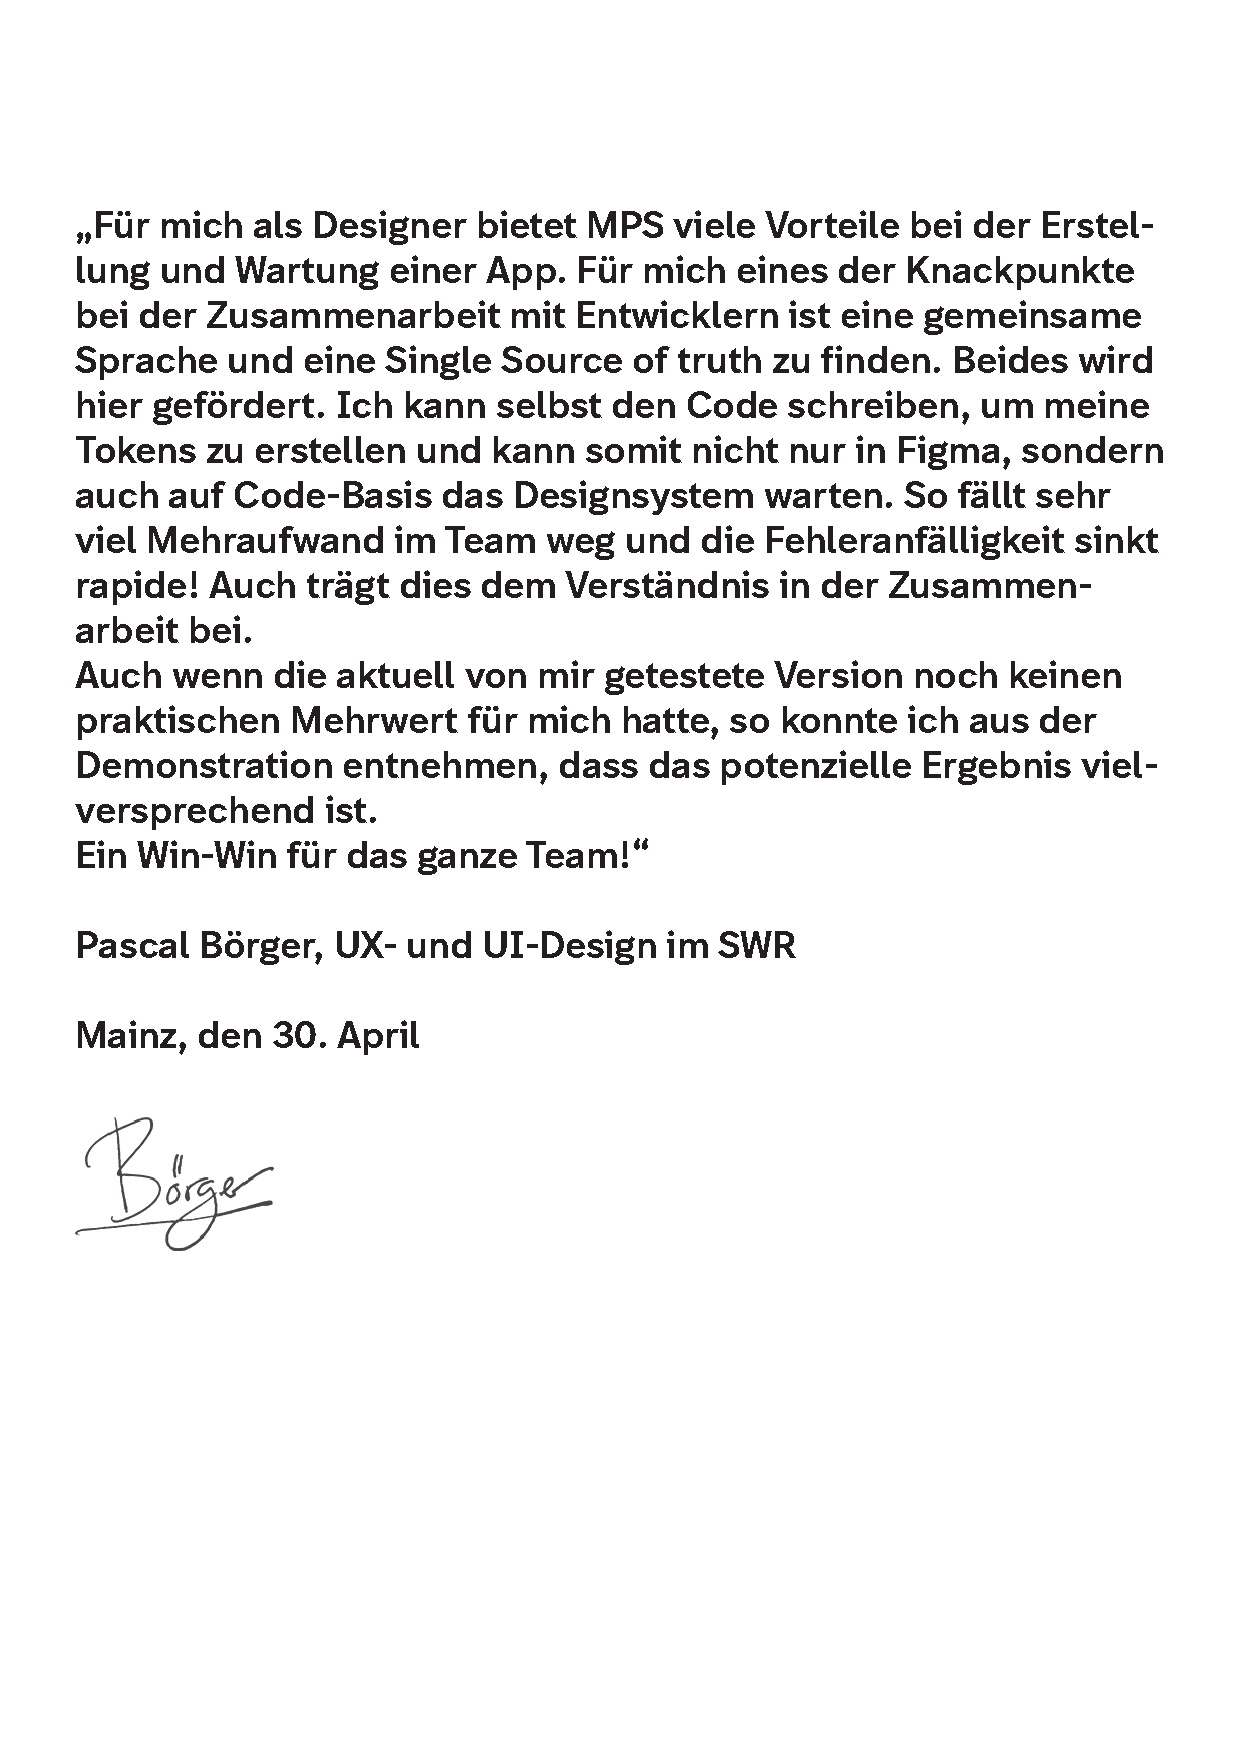
\includepdf[addtotoc={1,subsubsection,1,Pascal Börger,appendix:pascal-borger},pagecommand={}]{../assets/appendix/feedback_pb}

\includepdf[addtotoc={1,subsubsection,1,Julian Hültenschmidt,appendix:julian-hultenschmidt},pagecommand={}]{../assets/appendix/feedback_jh}

\includepdf[addtotoc={1,subsubsection,1,Bayram Ünlü,appendix:bayram-unlu},pagecommand={}]{../assets/appendix/feedback_bu}

\subsection{Eidesstattliche Versicherung}\label{appendix:eidesstattliche-versicherung}
Hiermit versichere ich an Eides statt, dass ich die vorliegende Bachelorarbeit mit dem Titel \enquote{\thetitle} selbstständig und ohne Hilfe Dritter verfasst habe.
Ich habe keine anderen als die angegebenen Hilfsmittel und Quellen benutzt.
Alle wörtlich oder sinngemäß übernommenen Textstellen habe ich als solche kenntlich gemacht.
Ich versichere, dass ich die Arbeit in dieser oder einer ähnlichen Form noch keiner anderen Prüfungsbehörde vorgelegt habe.
Mir ist bekannt, dass bei einem Verstoß gegen diese Grundsätze die Arbeit als nicht bestanden bewertet werden kann.

\vfill

\noindent Ort, Datum: Dorsten, \today \hspace{1cm} Unterschrift: \hrulefill           \\
\phantom{Ort, Datum: Dorsten, \today \hspace{1cm} Unterschrift:} \theauthor
